\documentclass{article}

\usepackage {booktabs}
\usepackage {tabularx}
\usepackage {graphicx}
\usepackage {float}

\title{Calling Bailey}
\author{ Team 5 \\ 
        William Tran \\
		Thien Trandinh \\
		Terrance Yip \\
		Susan Yuen}
\date{\today}

\begin{document}

\maketitle
\newpage
\tableofcontents
\listoffigures

\newpage

\section {General Information}

\subsection{Description}

The system is designed to take user inputted queries about the state of the ocean, and return it in a timely manner.

\subsection{Purpose}

The purpose is for those stranded in the ocean to have a means of receiving information to better their chances of survival through receiving information about the current status of the ocean. These properties include weather, ocean current waves, and other warnings.

\subsection{Scope}

The scope is a finite range of the ocean such that all other systems are within range.

\section{Module Hierarchy}
This section provides the hierarchy of the modules that will be implemented, from bottom up.

\begin{itemize}
    \item M1: Receiving Module
    \item M2: Data Processing module
    \item M3: Data Acquisition Module
    \item M4: Reply Module
\end{itemize}

\section{System Architecture}

\begin{figure}[H]
    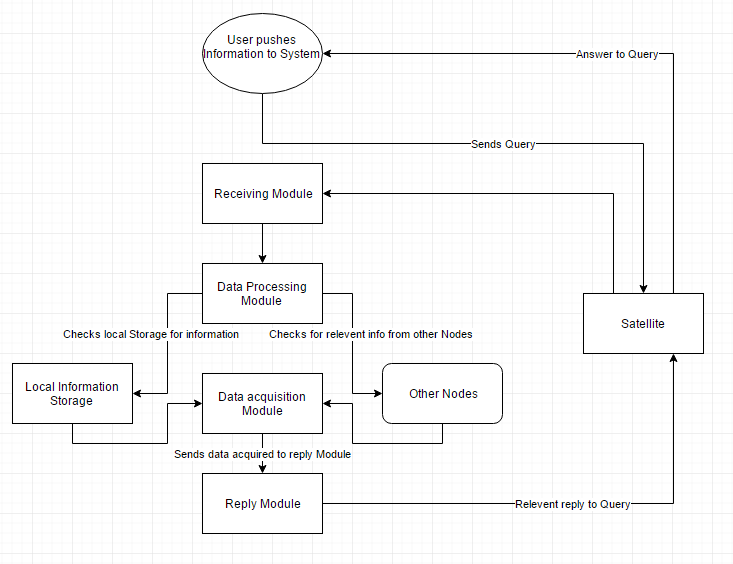
\includegraphics[width=\linewidth]{model.png}
    \caption {System Architecture}
    \label {fig:system}
\end{figure}

\section {Requirements}
\subsection{Assumptions}
The requirements for the system are based off the following assumptions:
\begin{itemize}
    \item The system receives messages from satellite phones through text messaging, and replies to the user through text messaging.
    \item All nodes contacting the system have a unique, immutable signature.
    \item The system has a reliable set of satellites that it has already established or may establish a connection to. The system is able to use these satellites to perform its duties.
    \item The weather node will update the system's weather log file.
\end{itemize}

\subsection{Functional Requirements}
\begin{enumerate}
    \item The system shall be able to take in user input through text messages.
    \item The system shall reply to the user through text messages.
    \item The system shall be able to decipher input messages into queries if possible, and shall notify the user if the message is invalid.
    \item The system shall support processing for queries of the type weather, warning, and current.
    \item For queries of type weather, the system shall reply to the user with an update of the latest weather status from the weather system.
    \item For queries of type warning, the system shall reply to the user with any warnings that have been sent within the past time period.
    \item For queries of type current, the system shall reply to the user with an update of the latest current status from the ocean current detection system.
    \item The system shall store logs for errors, weather, warnings, and ocean currents.
    \item The system shall have an option for the user to request instructions on how to use the system.
\end{enumerate}

\subsection{Non-Functional Requirements} 
\begin{enumerate}
    \item The system shall process queries quickly
    \item The system shall reply back to the caller quickly
    \item The system shall have easy instructions to follow in the help messages
    \item The system shall be easy to access
\end{enumerate}

\section {Traceability Matrices}
\subsection{Trace Between Requirements and Modules}

{\renewcommand{\arraystretch}{1.4}
\begin{tabularx}{\textwidth}{lX}
    \toprule
	\textbf{Requirements} & \textbf{Modules} \\
	\midrule
    \textbf{R1} & M1 \\
    \textbf{R2} & M4 \\
    \textbf{R3} & M2, M4 \\
    \textbf{R4} & M2 \\
    \textbf{R5} & M2, M4 \\
    \textbf{R6} & M2, M4 \\
    \textbf{R7} & M2, M4 \\
    \textbf{R8} & M3 \\
    \textbf{R9} & M1, M2, M4 \\
	\bottomrule
\end{tabularx}

\section{Waiting Room}

Due to time constraints, we were unable to finish implementing the following classes:\\
Query\\
QueryType\\
QYeryWhen\\
Store\\
 due to not having finished the required stubs for simulations\\
 
 
 \section{Features}
 The following are implemented:\\
 Ping from satellite\\
 picking best satellite in according to ping\\
 user input
 
 


\end{document}